% !TeX program = xelatex
% !TeX spellcheck = de_DE
\documentclass{beamer}
\usepackage{fontspec}
\usepackage{polyglossia}
\usepackage[notocbib]{apacite}
\usepackage{hyperref}
\usepackage{xspace}
\usepackage{array}
\usepackage{fontawesome}
\usepackage[normalem]{ulem}

% taken from http://tex.stackexchange.com/questions/45912/box-around-a-few-items-in-an-itemize-environment

\usepackage{xparse}%  For \NewDocumentCommand
\usepackage{calc}%    For the \widthof macro
\usepackage{tikz}
\usetikzlibrary{calc}

\newcommand{\tikzmark}[1]{\tikz[overlay,remember picture] \node (#1) {};}

\NewDocumentCommand{\DrawBoxWide}{s O{}}{%
    \tikz[overlay,remember picture]{
    \IfBooleanTF{#1}{%
        \coordinate (RightPoint) at ($(left |- right)+(\linewidth-\labelsep-\labelwidth,0.0)$);
    }{%
        \coordinate (RightPoint) at (right.east);
    }%
    \draw[red,#2]
      ($(left)+(-\labelwidth,0.9em)$) rectangle
      ($(RightPoint)+(0.2em,-0.3em)$);}
}

\setsansfont{Calibri}
\setdefaultlanguage{german}
\usetheme{UHH}

\def\authors#1#2{\author[#1]{#2}}
\def\email#1{\texttt{#1}}
\title{Microservices und Sicherheit}
\subtitle{Seminar Komponenten, Agenten und Workflows in verteilten Systemen}
\authors{Felix Ortmann \& Konstantin~Möllers}{Felix~Ortmann und Konstantin~Möllers\\ \email{\{0ortmann,1kmoelle\}@informatik.uni-hamburg.de}}
\institute{Universität Hamburg\\Fachbereich Informatik\\Vogt-Kölln-Straße 30\\22527 Hamburg}


\date{16. Januar 2016}
\titlegraphic{
\includegraphics[width=3cm]{img/uhh.pdf}}

\renewcommand{\APACrefauthstyle}{\bfseries}
\setcounter{tocdepth}{1}
\def\tocname{Gliederung des Vortrags}
\AtBeginSection{\frame{\frametitle{\tocname}\tableofcontents[currentsection]}}

\newcolumntype{x}[1]{>{\centering\arraybackslash}m{#1}}
\setbeamertemplate{headline}[default]

\defbeamertemplate*{title page}{customized}[1][]
{
	{\color{leuchtrot}
	\usebeamerfont{title}\centering\inserttitle\par
	\centering\usebeamerfont{subtitle}\insertsubtitle\par}
	\bigskip
	\centering\usebeamerfont{author}\insertauthor\par
	\bigskip
	\usebeamerfont{institute}\insertinstitute\par
	\bigskip
	\usebeamerfont{date}\insertdate\par
}

\begin{document}

\fontsize{14pt}{14pt}
	
% Titelfolie
{\setbeamercolor{title page}{bg=leuchtrot}
\begin{frame}%
	\titlepage
\end{frame}}

% Gliederung
\begin{frame}{\tocname}
	\tableofcontents
\end{frame}

\section{Einführung}

\subsection{Eigenschaften von Microservices}
\begin{frame}{\insertsubsection}
	\begin{columns}[T]
		\begin{column}{.33\linewidth}
			\centering
			
\includegraphics[width=.8\linewidth,page=1]{img/features}\\
			„gleiches zu gleichem!“
		\end{column}
		\begin{column}{.33\linewidth}
			\only<2->{
			\centering
			
\includegraphics[width=.8\linewidth,page=2]{img/features}\\
			„le Service c'est moi!“}
		\end{column}
		\begin{column}{.33\linewidth}
			\only<3->{
			\centering
			
\includegraphics[width=.8\linewidth,page=3]{img/features}\\
			„toll, ein anderer macht's!“}
		\end{column}
	\end{columns}
	\vfill
	\hfill{\footnotesize\cite{Fowler+14}}
\end{frame}

\subsection{Abgrenzung}
\begin{frame}{\insertsubsection}
	\begin{itemize}
		\item \textbf{SOA}\\
		fehlt: gekapseltes Frontend.\\
		hier: klare Trennung der Systeme, generische Schnittstelle durch das Web.
		
		\item \textbf{MAS}\\
		fehlt: soziologische Theorie.\\
		hier: soziotechnische Perspektive.
		
		\item \textbf{MOrgaS} \cite{Wester-Ebbinghaus10} \\
		fehlt: Schachtelbarkeit und Hierarchie.\\
		hier: Föderalismus, dezentralisierte Governance.
	\end{itemize}
\end{frame}

\definecolor{greenc}{HTML}{00AB84}
\definecolor{redc}{HTML}{EF3340}

\def\Plus{\color{greenc}+}
\def\Minus{\color{redc}–}
\subsection{Für und Wider}
\begin{frame}{\insertsubsection}
	\begin{columns}
		\begin{column}{.5\linewidth}
			\centering\textbf{\textcolor{greenc}{Pro}}
			\begin{itemize}
				\item[\Plus] Skalierbarkeit auf Enterprise-Ebene
				\item[\Plus] höhere Entscheidungsbefugnis für Entwickler
				\item[\Plus] \textit{Rapid Prototyping} von Anwendungen möglich
				\item[\Plus] schnellerer Zugang zu neuen Technologien und Programmiersprachen
			\end{itemize}
		\end{column}
		\begin{column}{.5\linewidth}
			\centering\textbf{\textcolor{redc}{Kontra}}
			\begin{itemize}
				\item[\Minus] hoher technischer Aufwand
				\item[\Minus] ausführliche Absprache und gute Tests obligatorisch
				\item[\Minus] Latenz und Overhead durch Kommunikation
				\item[\Minus] übergreifendes System-Refactoring schwer bis unlösbar
			\end{itemize}
		\end{column}
	\end{columns}
	
\end{frame}

\subsection{Motivation: Microservices + Sicherheit}
\begin{frame}{\insertsubsection}
	\begin{itemize}
		\item unabhängige, kleine Teams
		\begin{itemize}
			\item[$\Rightarrow$] bessere, leichtere Kommunikation
			\item[$\Rightarrow$] effizientes Debugging und Pair-Programming
		\end{itemize}
		\item Unabhängigkeit der Ausführung von Services
		\begin{itemize}
			\item[$\Rightarrow$] Hoheit über eigene Software
			\item[$\Rightarrow$] rasches, häufiges Deployment und schließen von Sicherheitslücken
		\end{itemize}
		\item einfache, generelle Schnittstelle
		\begin{itemize}
			\item[$\Rightarrow$] viele gut getestete Tools für die Kommunikation
			\item[$\Rightarrow$] Skalierung leichter und schneller möglich
		\end{itemize}
	\end{itemize}
\end{frame}

	
\section{Microservice-Architekturen und Sicherheit}

\subsection{Technologien zur Realisierung von MS}
\begin{frame}{\insertsubsection}
	\begin{itemize}
		\setlength\itemsep{2em}
		\item Köhasion, Autonomie, Kooperation wahren und unterstützen
		\item softwaretechnisch: \textit{Isolation} \& \textit{Kapselung}
		\item System formen aus einzelnen „Bausteinen“
		\item virtuelle Maschinen \& Container
	\end{itemize}
\end{frame}

\subsection{VMs \& Container}
\begin{frame}{\insertsubsection}
	Virtuelle Maschine
	\begin{itemize}
		\setlength\itemsep{1em}
		\item isoliert Anwendung(en)
		\item „sandboxed“ Execution Environment
		\item Anwendung $\approx$ VM-Image $\rightarrow$ Replizierbar
		\item „schwer“
		\begin{itemize}
			\item[$\Rightarrow$] beinhaltet eigene Libs und Gast-Betriebssystem
			\item[$\Rightarrow$] Images meist groß
		\end{itemize}
	\end{itemize}
\end{frame}

\subsection{VMs \& Container}
\begin{frame}{\insertsubsection}
	Container (insb. Docker)
	\begin{itemize}
		\setlength\itemsep{1em}
		\item isoliert genau eine Anwendung
		\item \textit{Namespaces}, \textit{Network Interfaces}, \textit{Cgroups}, \textit{Chroots}
		\item Replikation via Dockerfile oder Image
		\item „leicht“
		\begin{itemize}
			\item[$\Rightarrow$] beinhaltet nur App und Abhängigkeiten
			\item[$\Rightarrow$] Images klein
			\item[$\Rightarrow$] Ausführung: 1 Prozess
		\end{itemize}
	\end{itemize}
\end{frame}

\subsection{VMs \& Container}
\begin{frame}{\insertsubsection}
	\centering
	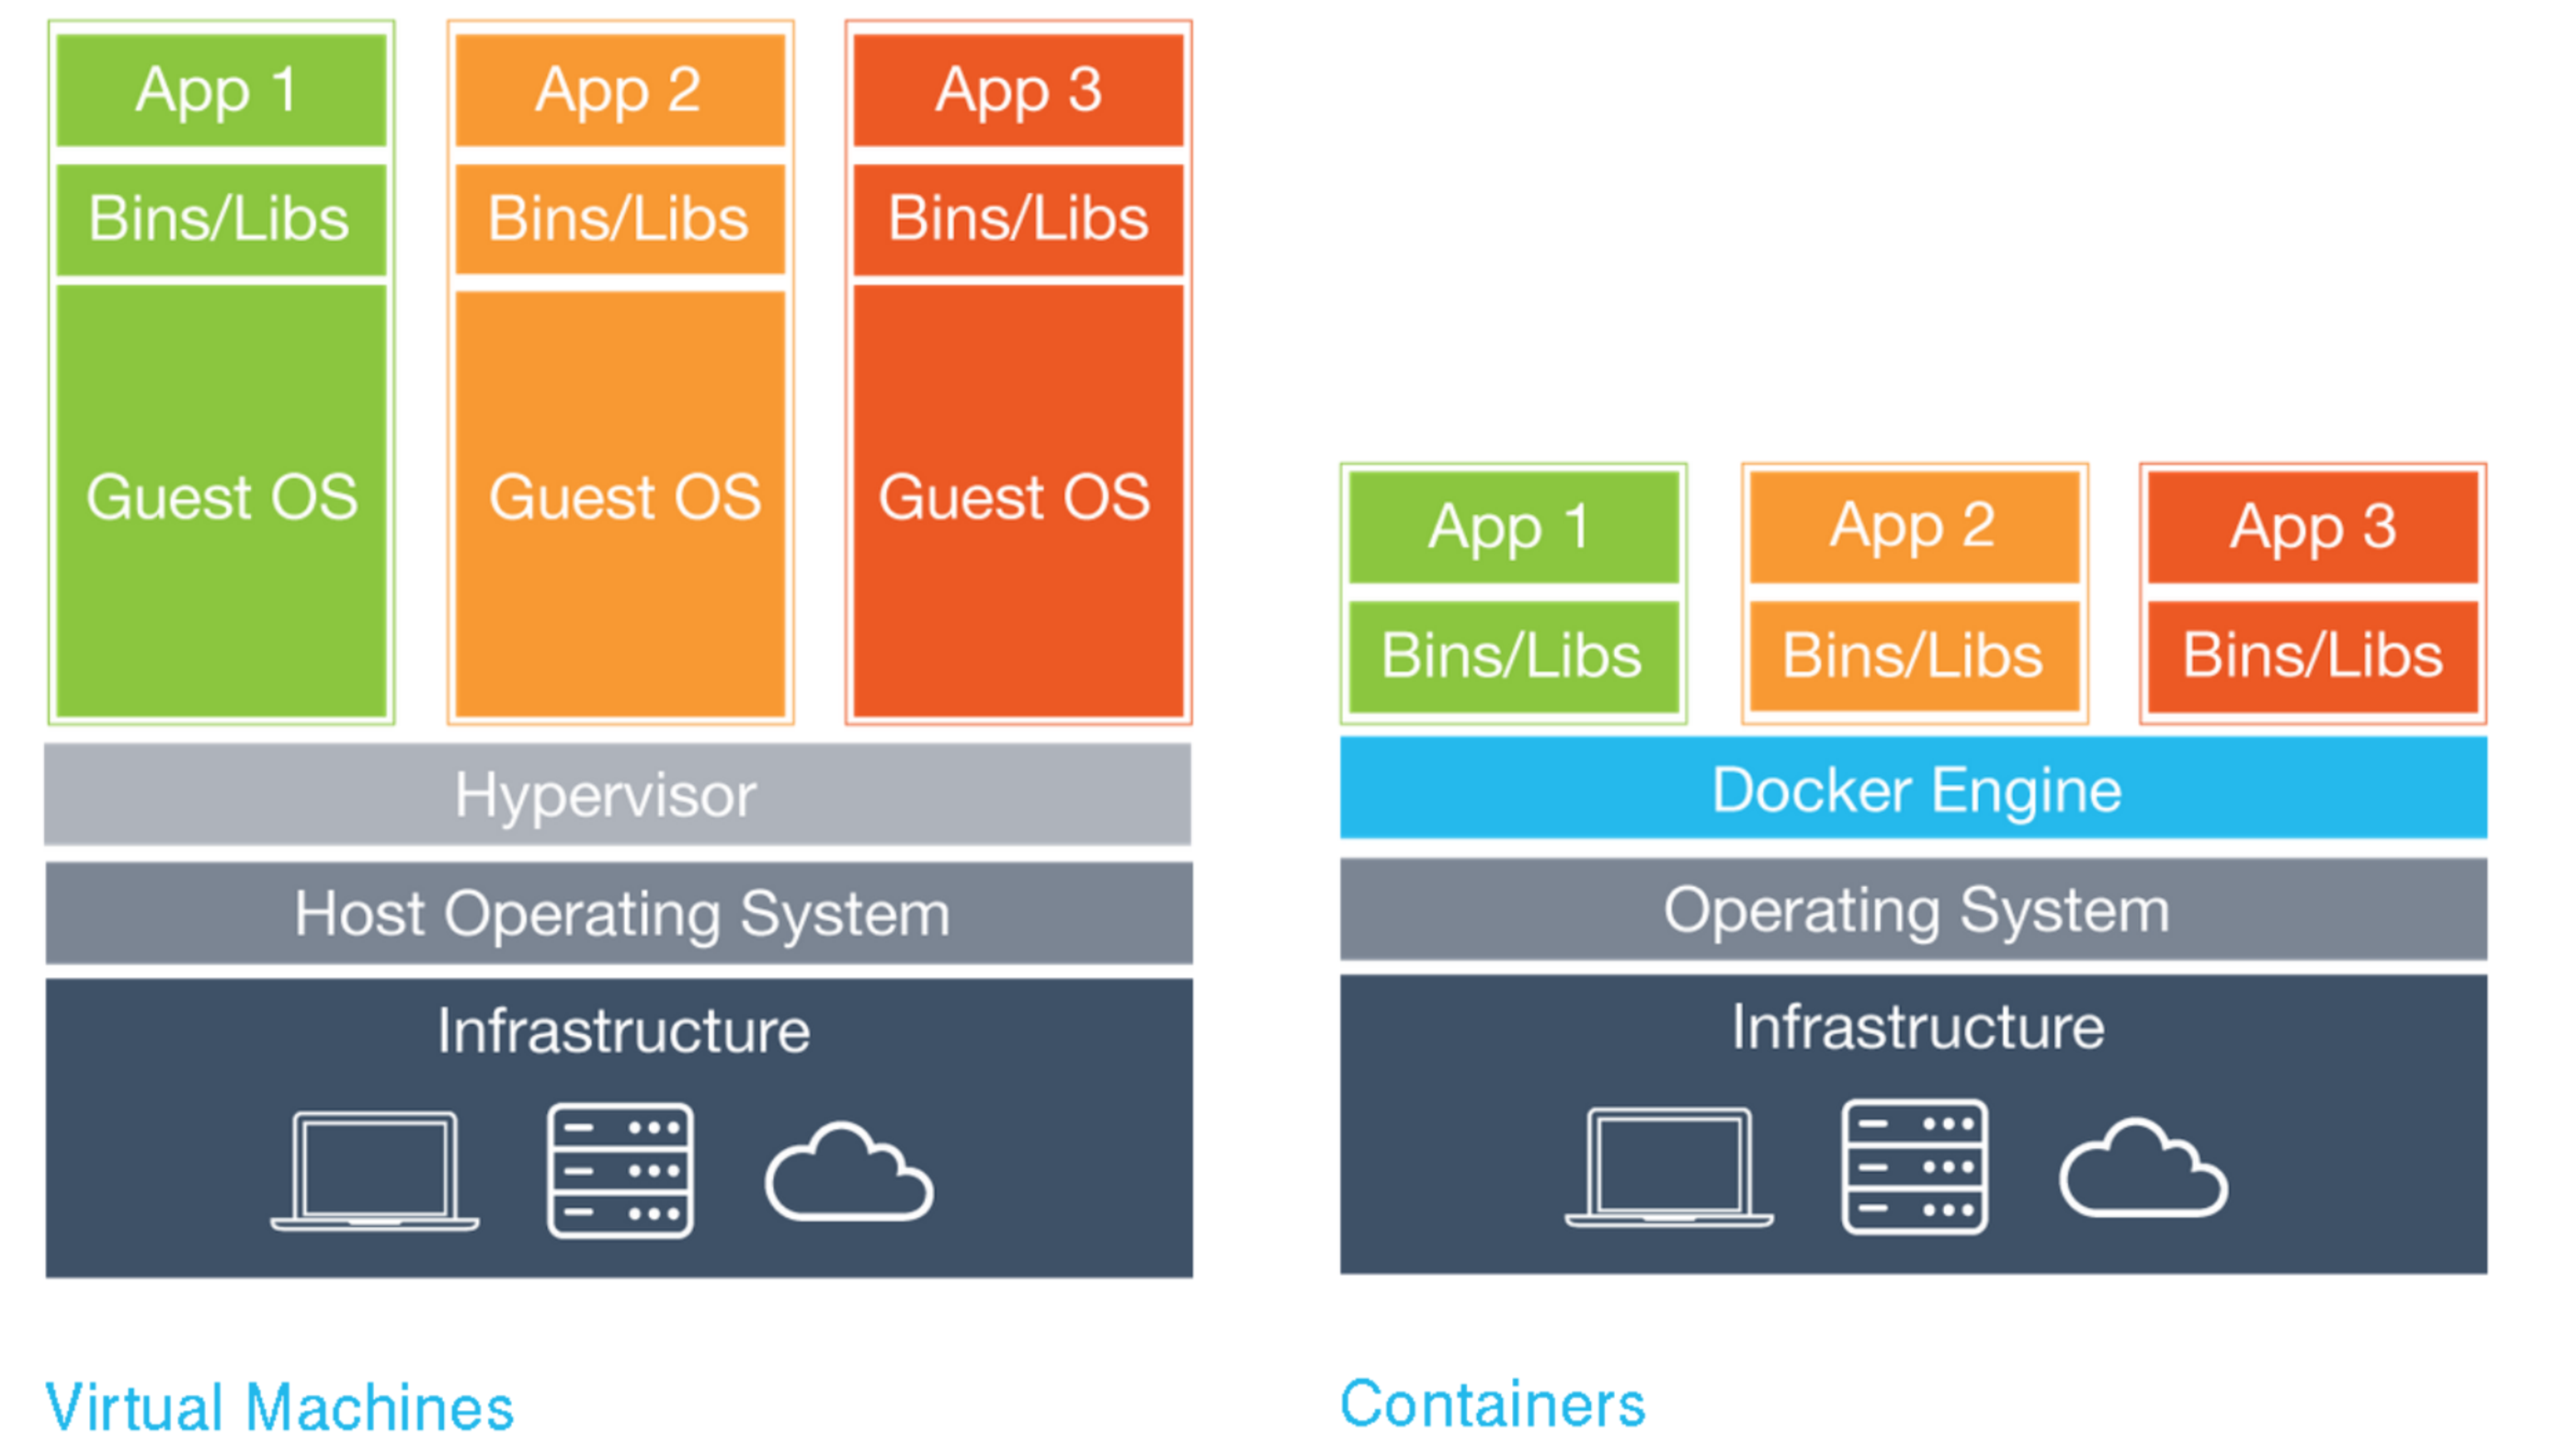
\includegraphics[width=\linewidth]{img/container-vm.pdf}
\end{frame}

\subsection{Microservice Systeme}
\begin{frame}{\insertsubsection}
	\begin{itemize}
		\item Zusammenspiel vieler Microservices
		\item „viele bewegliche Teile“ $\rightarrow$ neue Probleme:
		\vspace*{1em}
		\begin{enumerate}
			\setlength{\itemindent}{6em}
			\setlength\itemsep{0.5em}
			\item \tikzmark{left}Service Discovery
			\item Erreichbarkeitsüberwachung
			\item Skalierbarkeit
			\item Load Balancing
			\item Deployment
			\item Replizier- \& Portier \& Ersetzbarkeit 
			\item Kommunikationssicherheit
			\item Verhaltensüberwachung (Logging)\tikzmark{right}
		\end{enumerate}
		\DrawBoxWide[thick, blue, fill=yellow, fill opacity=0.2]
		\item „Orchestration“: \textit{K8s}, \textit{Mesos}, \textit{ECS}, \textit{Azure} ...
	\end{itemize}
\end{frame}

\subsection{Kubernetes}
\begin{frame}{\insertsubsection}
	\centering
	
\includegraphics[width=.3\linewidth]{img/kubernetes_logo.png}
	\vspace*{1em}

	\textit{„Kubernetes is an open-source platform for automating deployment, scaling, and operations of application containers across clusters of hosts.“}\cite{k8sdoc}
	\vspace*{1em}	
	\begin{itemize}
		\setlength\itemsep{1em}
		\item löst obige Problemstellungen 1-7
		\item abstrahiert Lösung, um mit Docker Containern MS Systeme zu realisieren
	\end{itemize}
\end{frame}

\subsection{Kubernetes}
\begin{frame}{\insertsubsection}
	\begin{itemize}
		\setlength\itemsep{1em}
		\item Pods
		\item Services
		\item Replication Controller
	\end{itemize}
	\vspace{1em}
	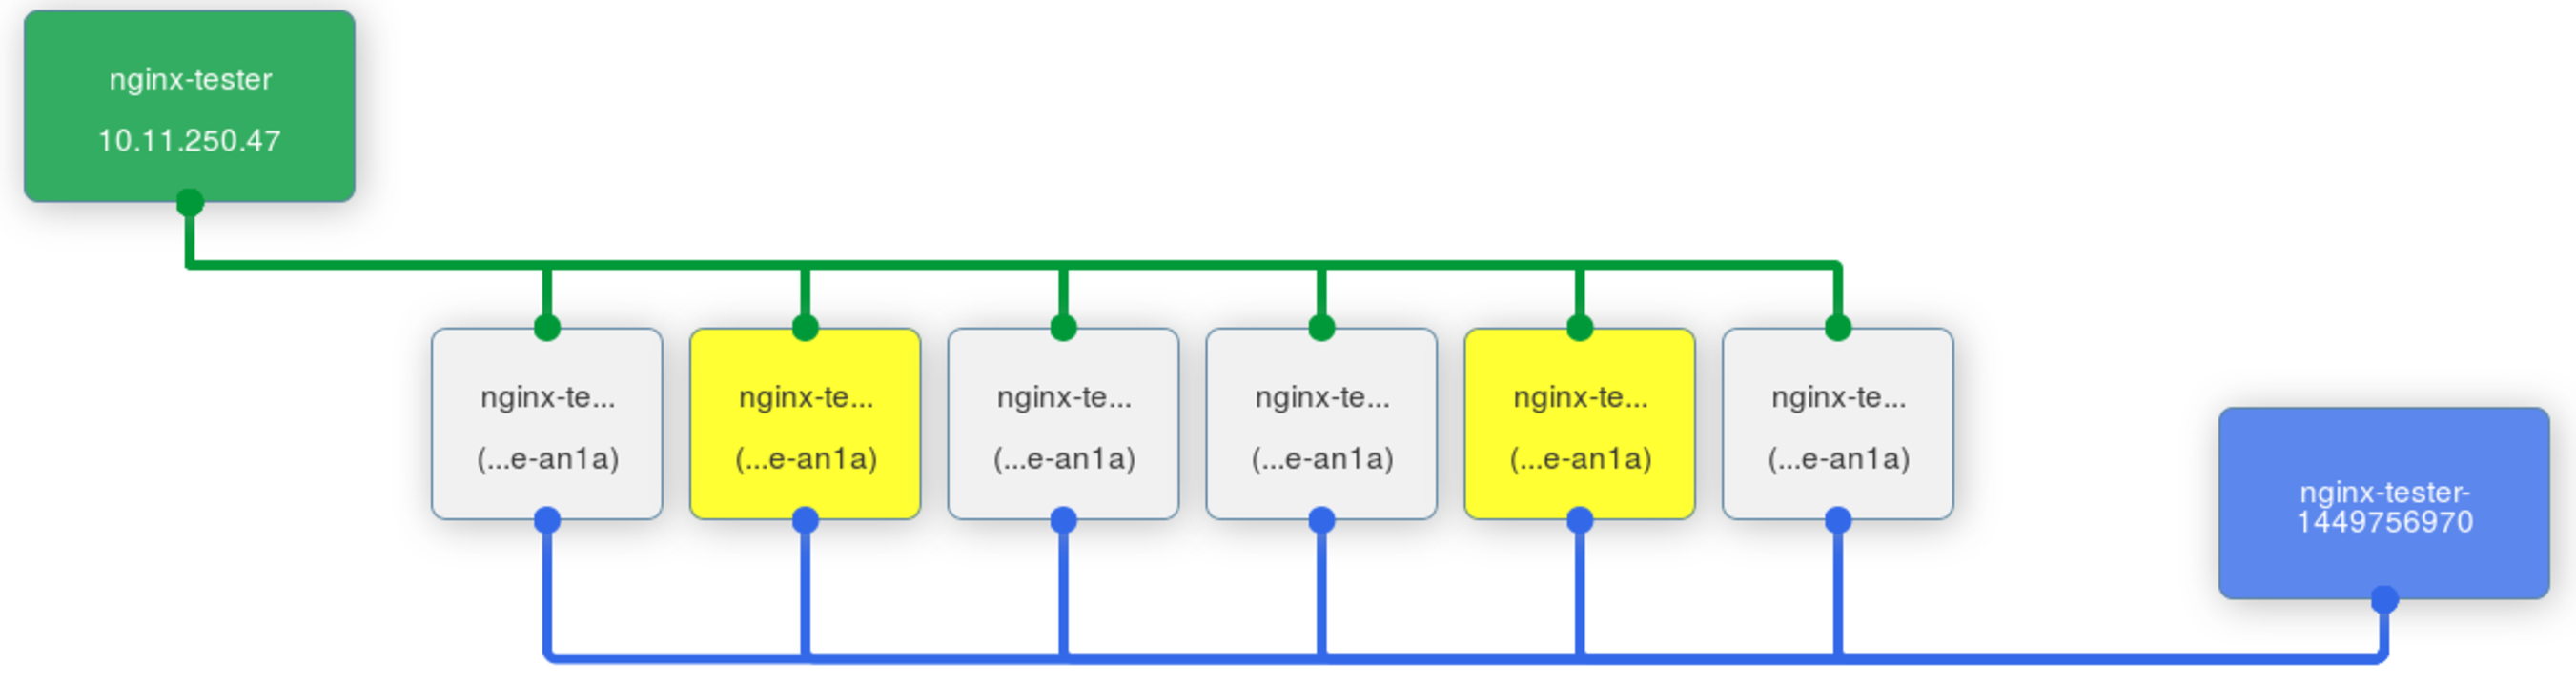
\includegraphics[width=\linewidth]{img/pods-getting-ready-k8s.pdf}
\end{frame}
		
\section{Kommunikation und Sicherheit}

\subsection{Kommunikationsbedarf}
\begin{frame}{\insertsubsection}
	\begin{itemize}
		\setlength\itemsep{1em}
		\item „System“ $\rightarrow$ Vernetzung der Microservices
		\item \textit{Orchestration Tools} versuchen, das Problem zu adressieren
		\item Kommunikation fast immer Event-basiert
		\item Technologien: REST \& Message Queues
		\item Problem: Unsichere Kanäle
	\end{itemize}
\end{frame}

\subsection{\em RESTful APIs}
\begin{frame}{\insertsubsection}
	\begin{itemize}
		\setlength\itemsep{1em}
		\item „Representational State Transfer“
		\item Request / Response (HTTP)
		\item synchron -- Gesprächspartner bekannt
		\item abhörbar, manipulierbar, offene APIs
		\item HTTPS $\rightarrow$ \sout{abhörbar, manipulierbar} \emph{offene APIs}
		\item Authentifizierung an API + HTTPS -- Mindestsicherheit nach \cite{newman2015}
	\end{itemize}
\end{frame}

\subsection{\em Message Queues}
\begin{frame}{\insertsubsection}
	\begin{itemize}
		\setlength\itemsep{2em}
		\item asynchron \& indirekt -- Empfänger evtl. unbekannt
		\item bessere Skalierbarkeit, Worker-Chains
		\item Transport von/zu Queue unsicher
		\item \textit{RabbitMQ}, \textit{ZeroMQ}
	\end{itemize}
\end{frame}

\subsection{\em System Sandboxing}
\begin{frame}{\insertsubsection}
	\begin{itemize}
		\setlength\itemsep{2em}
		\item Gesamtsystem hinter Firewall
		\item Subnetze verwenden
		\item keine Schnittstelle zum WWW
		\item verlagert den Angriffsvektor, eliminiert ihn nicht!
	\end{itemize}
\end{frame}


\subsection{Validierung und Verifikation}
\begin{frame}{\insertsubsection}
	\begin{itemize}
		\setlength\itemsep{1em}
		\item Grobe Maßnamen:
		\begin{itemize}
			\item[$\Rightarrow$] Geteiltes JSON Schema
			\item[$\Rightarrow$] Hashing des Inhalts
			\item[$\Rightarrow$] Identifikation des Absenders
		\end{itemize}
		\item Im Detail: 
		\begin{itemize}
			\item[$\Rightarrow$] Pro Anwendungsfall Schutzziele definieren
			\item[$\Rightarrow$] Passende Technologie pro Schutzziel
			\item[$\Rightarrow$] Erhöhter Implementationsaufwand wenn richtig gemacht
		\end{itemize}
	\end{itemize}
\end{frame}

\section{Schutzziele}

\subsection{Vertraulichkeit}
\begin{frame}{\insertsubsection}
	\begin{itemize}
		\setlength\itemsep{1em}
		\item Informationen nur Befugten zugänglich
		\item Informationsflüsse festlegen und kontrollieren
	\end{itemize}
	\vspace*{1cm}
	\pause
	Vorgestellte Verfahren:
	\begin{itemize}
		\item \textit{OAuth}
		\item \textit{JSON Web Tokens}
	\end{itemize}
\end{frame}

\subsection{\em OAuth 2}
\begin{frame}{\insertsubsection}
	\centering
	
\includegraphics[width=.3\linewidth]{img/oauth}
	\vspace*{12pt}
	\begin{itemize}
		\item RFC 6749 \cite{RFC6749}
		\item ermöglicht \textit{Single Sign On}
		\item basiert auf Web-Technologie (vor allem HTTP)
		\item vielfach genutzt, z.B. von Google, Facebook, …
	\end{itemize}
\end{frame}	

\begin{frame}{\insertsubsection}
	\begin{figure}
		\centering
		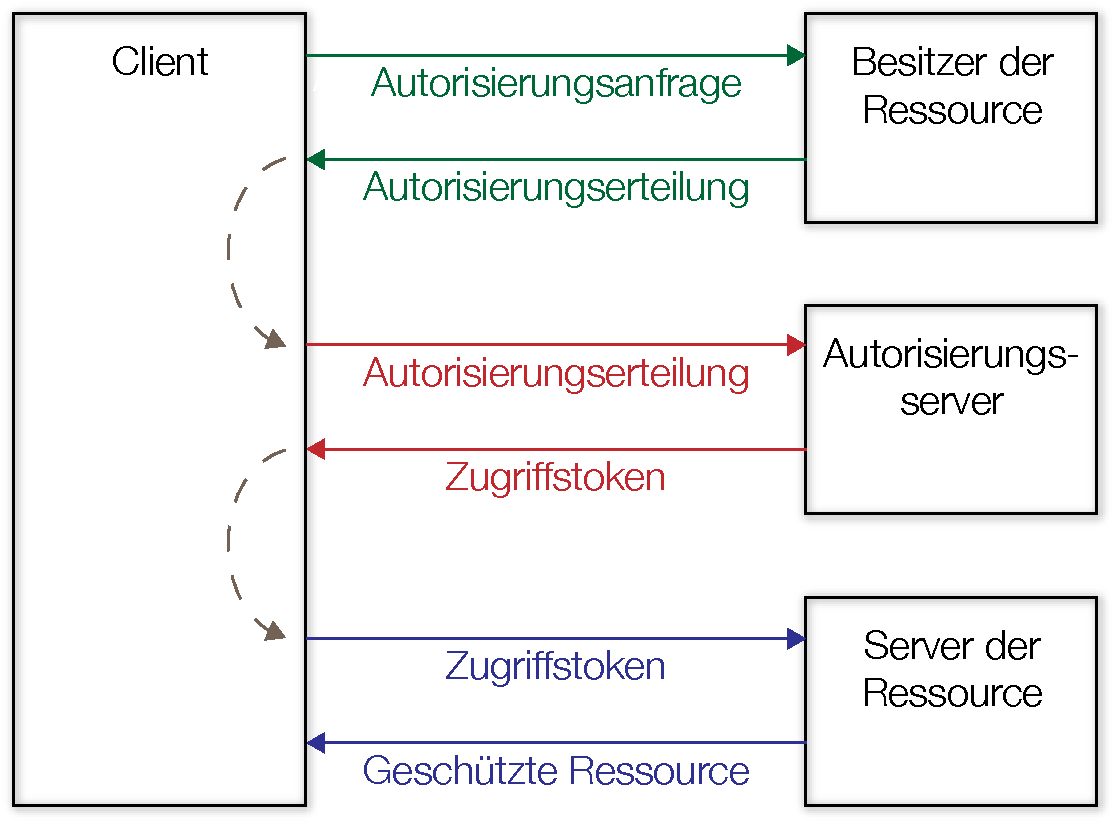
\includegraphics[width=.52\linewidth]{img/OAuth2}
		\caption{Protokollablauf bei OAuth 2 (übersetzt aus RFC 6749)}
	\end{figure}
\end{frame}
	
\subsection{\em JSON Web Tokens}
\begin{frame}{\insertsubsection}
	\centering
	
\includegraphics[width=.5\linewidth]{img/jwt}
	\vspace*{12pt}
	\begin{itemize}
		\item RFC 7519 \cite{RFC7519}
		\item simpler gegenüber \textit{OAuth}
		\item jeder Client kann verifizieren
		\item klein, daher via HTTP übertragbar
		\item kann auch von Browsern geparsed werden
	\end{itemize}
\end{frame}
	
\begin{frame}{\insertsubsection}{}%

\begin{figure}
	\framebox[.8\linewidth]{\parbox{.75\linewidth}%
{\color{red}\tt\footnotesize\{\\
		\hspace*{2em}"alg": "RS256",  \textcolor{gray}{// Verschlüsselungsalgorithmus}\\
		\hspace*{2em}"typ": "JWT" \textcolor{gray}{// „JSON Web Token“, offen für weitere}\\
\}}}
\caption{JWT-Header}
\end{figure}

\begin{figure}
	\framebox[.8\linewidth]{\parbox{.75\linewidth}%
{\color{violet}\tt\footnotesize\{\\
		\hspace*{2em}"thema": "Microservices und Sicherheit",\\
		\hspace*{2em}"modul": "Entwicklung verteilter Systeme",\\
		\hspace*{2em}"kursnr": "64-400"\\
	\}}}
\caption{JWT-Payload}
\end{figure}

\end{frame}

\begin{frame}{\insertsubsection}
	\begin{figure}
		{\tt \textcolor{red}{
				eyJhbGciOiJSUzI1NiIsInR5cCI6IkpXVCJ9}.\textcolor{violet}{eyJ0aG\\
				VtYSI6Ik1pY3Jvc2VydmljZXMgdW5kIFNpY2hlcmhla\\
				XQiLCJtb2R1bCI6IkVudHdpY2tsdW5nIHZlcnRlaWx0\\
				ZXIgU3lzdGVtZSIsImt1cnNuciI6IjY0LTQwMCJ9}.\textcolor{blue}{gb\\
				0y7zl4-IIZrRdWD14UaSGPz34vXqAPecoyQVeOrntFx\\
				PSkhryDHn2ts3Wn7XyHjli1HDdLZbqV5f1SzHNKZfz\_\\
				Ww8Tl2xzKLURpX9QxuI2PvFQZF0bQ7PeKqmZD7OU4eI\\
				4y9L6srzedEjsDDISbaFXTaIJp\_j1JtM9XTtEgi2Vy9\\
				TAIZczCacnxuJgxd-Nk40k6KgnFPz1ETIu9G3JyyMxP\\
				Enh1pw7EzIefJnRaaswC0K1evjQFK6dFvIlgXuevM3u\\
				gZcI7lA2f1PeMud1fkZu3yaw27jeeLZRU1WiRhMV9EB\\
				5elsYiscnpoVjuEk4C8T-p3oji43zf1IT7XvBiQ}}
		\caption{Vollständiges \textit{JSON Web Token}}
	\end{figure}
\end{frame}

\subsection{Integrität}
\begin{frame}{\insertsubsection}
	\begin{itemize}
		\setlength\itemsep{1em}
		\item \textbf{Datenintegrität}:\\
			Vollständigkeit \& Korrektheit der Daten
		\item \textbf{Systemintegrität}:\\
			korrekte Funktionsweise des Systems
	\end{itemize}
	\vspace*{2em}
	\pause
	Vorgestellte Verfahren:
	\begin{itemize}
		\item Verschlüsselung
		\item Integrationstests
	\end{itemize}
\end{frame}

\subsection{Verschlüsselte Protokolle}
\begin{frame}{\insertsubsection}
	\begin{itemize}
		\item \textbf{HTTPS} – \textit{HyperText Transport Protocol Secure}
		\begin{itemize}
			\item RFC 2818
			\item sichere Übertragung von Daten + Informationen
		\end{itemize}
		\item \textbf{WSS} – \textit{WebSockets Secure}
		\begin{itemize}
			\item RFC 6455
			\item sichere und schnelle Übertragung von Daten in einem Socket
		\end{itemize}
		\item \textbf{SSH} – \textit{Secure Shell}
		\begin{itemize}
			\item RFC 42\{50-56\}
			\item sichere entfernte Ausführung via RSA und AES
		\end{itemize}
		\item \textbf{SFTP} – \textit{SSH File Transfer Protocol}
		\begin{itemize}
			\item (Working draft)
			\item sichere Übertragung von Dateien
		\end{itemize}
	\end{itemize}
\end{frame}

\subsection{Integrationstests für Microservices}
\begin{frame}{\insertsubsection}
	\begin{figure}[h]
		\centering
		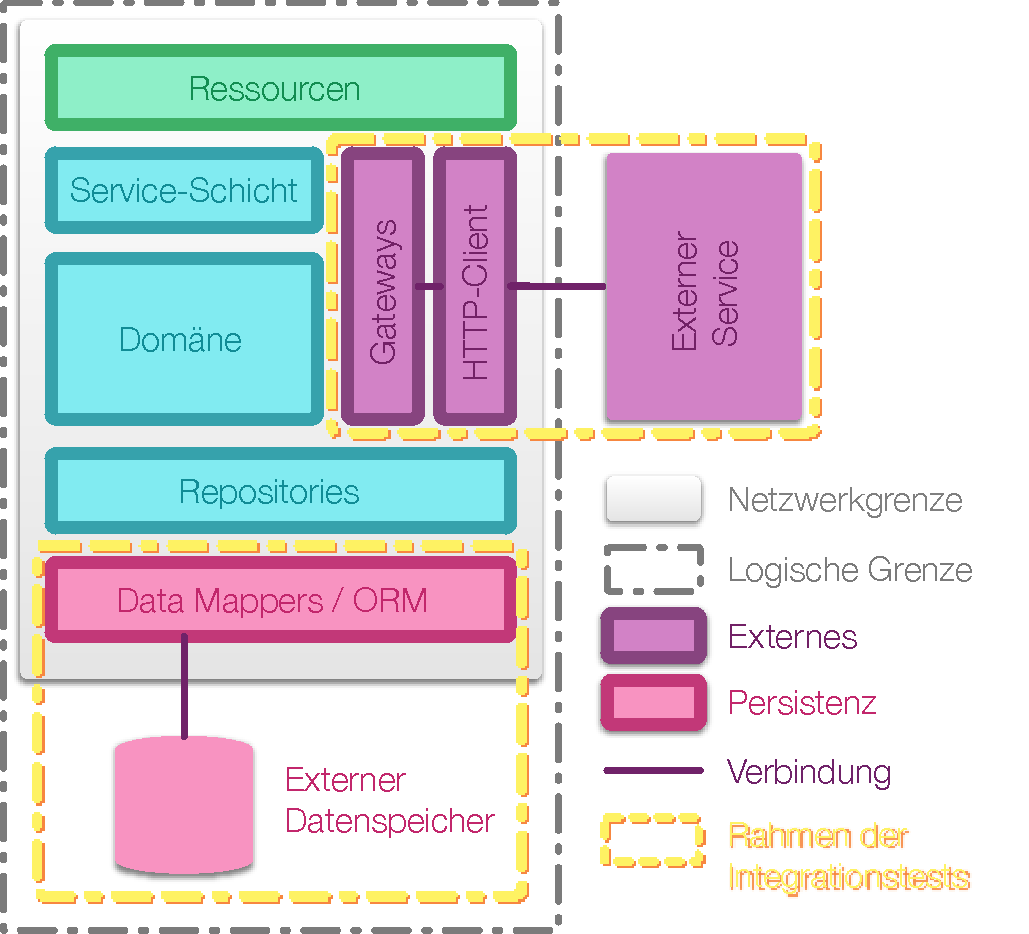
\includegraphics[width=.6\linewidth]{img/inte}
		\caption{Integrationstests in einer Microservice-Architektur (Clemson, 2014)}
		\label{fig:integrationstests}
	\end{figure}
\end{frame}

\subsection{Verfügbarkeit}
\begin{frame}{\insertsubsection}
	\begin{itemize}
		\setlength\itemsep{1em}
		\item Systeme stets betriebsbereit
		\item zeitgerechter Zugriff auf Daten jederzeit möglich
	\end{itemize}
	\vspace*{1cm}
	\pause
	Vorgestellte Verfahren:
	\begin{itemize}
		\item horizontale Skalierung \& Lastverteilung
		\item \textit{Baker Street}
	\end{itemize}
\end{frame}


\subsection{Horizontale Skalierung \& Lastverteilung}

\begin{frame}{\insertsubsection}
	\begin{columns}[T]
		\begin{column}{.5\textwidth}
			\centering
			\includegraphics[width=.6\textwidth, page=2]{img/scale-up-out.pdf}
			
			\textbf{\large\color{leuchtrot} Scale Up}
			
			\textit{„größere Box“}
			\begin{itemize}
				\item Hardwarekapazität erweitern (CPU, RAM, …)
				\item einfach \& günstig
				\item \textit{Single Point of Failure}
				\item unterliegende Software muss auch skalieren
			\end{itemize}
		\end{column}
		\begin{column}{.5\textwidth}
			\centering
			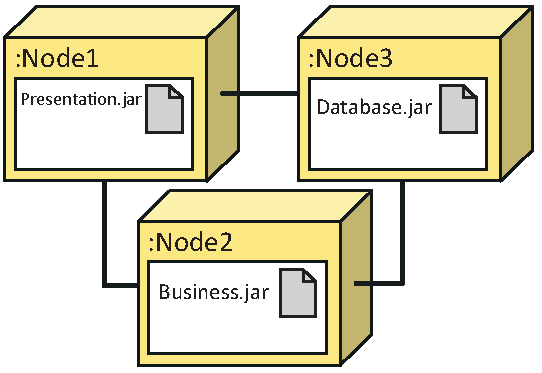
\includegraphics[width=.6\textwidth, page=1]{img/scale-up-out.pdf}
			
			\textbf{\large\color{leuchtrot} Scale Out}
			
			\textit{„mehr Boxen“}
			\begin{itemize}
				\item mehr Server hinzufügen und Lastverteilung
				\item schützt vor Hardwarefehlern
				\item leicht für die Microservice-Architektur!
			\end{itemize}
		\end{column}
	\end{columns}
	\vfill
	\hfill{\footnotesize\cite{Meier+08}}
\end{frame}
	
\begin{frame}{Arten von Lastverteilung}
	\begin{itemize}[<+->]
		\setlength\itemsep{1em}
		\item \textbf{Zufall} 
		\begin{itemize}
			\item einen zufälligen Knoten wählen
			\item sehr simpel, aber asymmetrisch
		\end{itemize}
		\item \textbf{Sharding} 
		\begin{itemize}
			\item Knoten auf Basis eines Indexes wählen
			\item bei guter Schlüsselwahl symmetrisch
		\end{itemize}
		\item \textbf{Auslastung} 
		\begin{itemize}
			\item Knoten mit geringster Auslastung wählen
			\item zusätzliche Belastung der Knoten
		\end{itemize}
	\end{itemize}
\end{frame}

\subsection{\em Baker Street}
\begin{frame}{\insertsubsection}
	\centering
	
\includegraphics[width=\linewidth]{img/bakerstreet}
	\begin{itemize}
		\item Open-Source-Projekt von 2015
		\item \url{http://bakerstreet.io/}
	\end{itemize}
\end{frame}

\begin{frame}{\insertsubsection}
	\begin{itemize}[<+->]
		\setlength\itemsep{1em}
		\item \textbf{Sherlock} 
		\begin{itemize}
			\item \textit{HAProxy}-basierter \textit{Load Balancer}
			\item lokal, findet andere Knoten
		\end{itemize}
		\item \textbf{Watson} 
		\begin{itemize}
			\item \textit{Health Checker}, prüft Zustand des Microservices 
			\item übernimmt Anmeldung
		\end{itemize}
		\item \textbf{Datawire-Verzeichnis} 
		\begin{itemize}
			\item globale Diensterkennung
			\item leitet Nachrichten von \textbf{Watson} an \textbf{Sherlock} weiter
		\end{itemize}
	\end{itemize}
	\vfill
	\hfill{\footnotesize\cite{Li15}}
\end{frame}

\begin{frame}{\insertsubsection}
	\begin{figure}
		\centering
		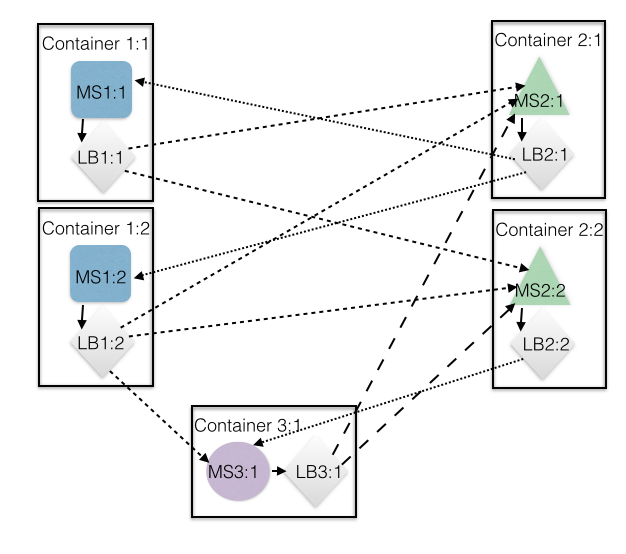
\includegraphics[width=.65\linewidth]{img/clientloadbal}
		\caption{Schematische Darstellung von clientseitiger Lastverteilung (aus Li, 2015)}
		\label{fig:clientseitige_lastverteilung}
	\end{figure}
\end{frame}

\section{Zusammenfassung}
\begin{frame}{\insertsection}
	\begin{itemize}
		\item Konzepte wie Kohäsion, Autonomie und Kooperation
		\item Container \& VMs
		\item Herausforderung: Zusammenspiel von MS
		\item Kommunikation via REST \& Queues
		\item Vertraulichkeit: \textit{OAuth 2} \& JWT
		\item Integrität: Verschlüsselung \& Tests
		\item Verfügbarkeit: \textit{Load Balancing} \& \textit{Baker Street}
	\end{itemize}
\end{frame}

\section{Demo und Diskussion}

% Literatur
\section{\bibname}
\begin{frame}[allowframebreaks]{\bibname}
	\AtBeginSection{}
	\nocite{*}
	\bibliographystyle{apacite}
	\bibliography{bib}
\end{frame}


\end{document}